\subsection{Configuration editor}
\writer{Monica}

The Configuration Editor is the component which allows the user to create a link between all the models that have been previously created with by using the other editors. The editor can be used by both technical and non-technical users since its main functionality is connecting the Petri net, the Geometry and the Appearance models. 

Figure \ref{fig:uml-configuration-editor} shows the model behind the Configuration Editor. 

\begin{figure}[htp]
\begin{center}
  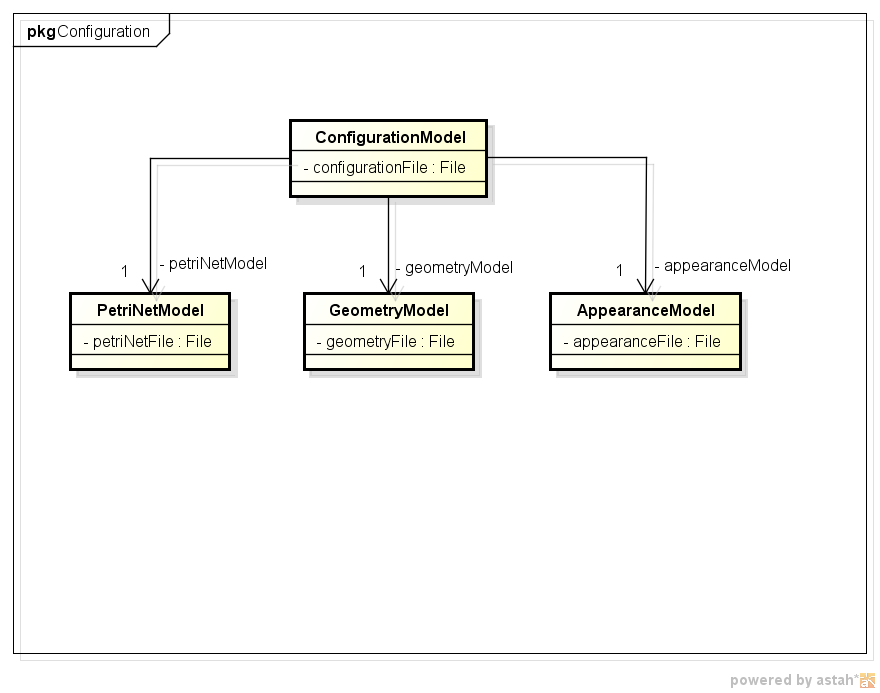
\includegraphics[width=0.8\textwidth]{image/configuration-model.png}
  \caption{UML for the Configuration Editor}
  \label{fig:uml-configuration-editor}
\end{center}
\end{figure}

\subsubsection{Configuration editor classes}

Next, a more detailed description of the model is provided.

\paragraph{ConfigurationModel}

The ConfigurationModel class has only one attribute, \textbf{configurationFile}, of type File, which will include all the information provided by the \textit{PetriNetModel}, \textit{GeometryModel} and \textit{AppearanceModel} objects. 

\paragraph{PetriNetModel}

The PetriNetModel class has only one attribute, \textbf{petriNetFile}, of type File, which represents the output file of the Petri net Editor. This file will include the description of all the objects in the petri net and their attributes. 

\paragraph{GeometryModel}

The GeometryModel class has only one attribute, \textbf{geometryFile}, of type File, which represents the output of the Geometry Editor. This file will include the description of all geometry objects and their attributes.

\paragraph{AppearanceModel}

The AppearanceModel class has only one attribute, \textbf{appearanceFile}, of type File, which represents the output of the Appearance Editor. This file will include the associations between appearance labels of the Petri net objects and their corresponding 3D objects or textures. 

